%\documentclass[main.tex]{subfiles}
%Edit
\lhead{Date taken: 1.22}
\chead{}
\rhead{Alice Michael}
\author{Alice Michael}
\title{CS410 Network Optimization Notes}
\date{}
\begin{document}

%\noindent\large{\bf \textit{Challenges}}\\

%\begin{figure}[h!]
%\centering
%\includegraphics[width=0.8\linewidth]{addressSpace.jpg}
%\caption[Address Space]{Address Space}
%\label{fig:Address Space}
%\end{figure}	

%\begin{enumerate}
%  \itemsep-1.5em
%  \item 
%\end{enumerate}


\section*{Presentations}

\section*{Diversity and Inclusion App}\\
Requirements:\\
\indent Develop a real time interactive solution focusing on employee engagement and Diversity and Inclusion\\

Skillset Recommended\\
\indent EQ (Emotional Intelligence) Software Development Social Media\\

\indent Not platform restricted\\

\indent This is a huuuuuuge open no expectations type project.  It's a very ambiguous project to increase diversity... Somehow.\\

\section*{Street Smart}
\indent Help a transportation and health nonprfit migrate a custom built website to an editable CMS for greater diffusion and ease of maintenance\\

\indent User information/profile, Community profiles\\
Welcome.thinkstreetsmart.org\\
Kelly Rodgers, Executive Director\\
kelly@thinkstreetsmart.org\\

\section*{Development of an app to report hate incidents in Portland}

\newpage
\section*{VA Tinnitus Care Plan}

Candice.Manning@va.gov\\
503-220-8262 x52448\\
https://www.ncrar.research.va.gov\\

There is a basic algorithmic thing in place.  With this, we will be testing and using different things\\
Project is already up on github to be worked on\\
This is a lot of background database work.  This would be to set up the database and connect with it.\\
Databases with input from the already existing forms\\
Tracking usability, feasability\\

\begin{figure}[h!]
\centering
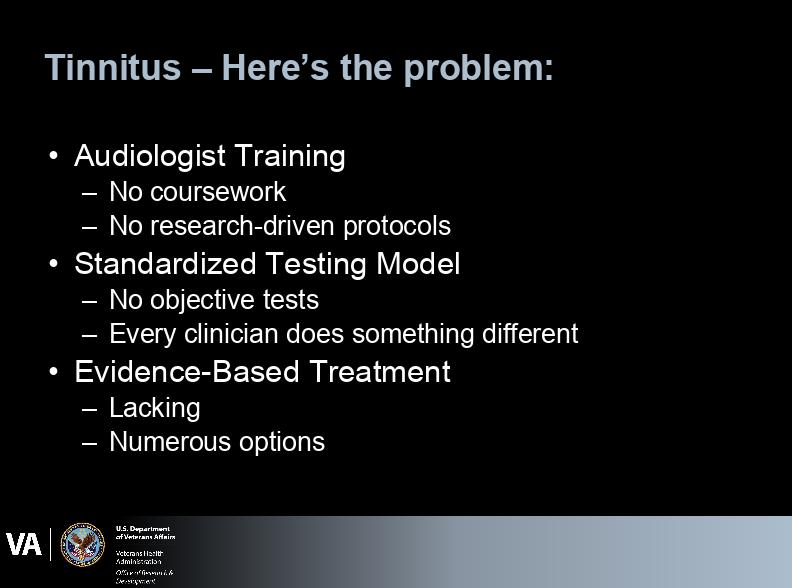
\includegraphics[width=0.8\linewidth]{P2-a.jpg}
\caption[VA]{VA}
\label{fig:VA}
\end{figure}	
\newpage
\begin{figure}[h!]
\centering
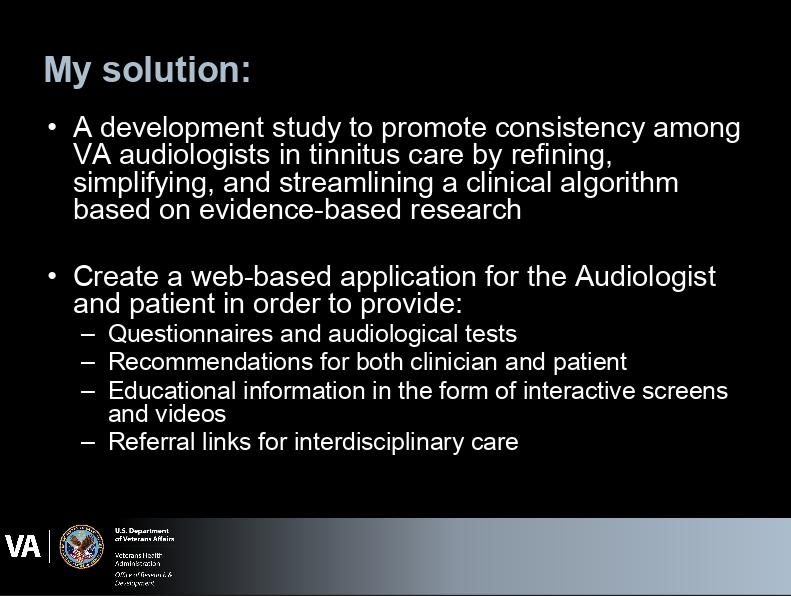
\includegraphics[width=0.8\linewidth]{P2-b.jpg}
\caption[VA]{VA}
\label{fig:VA}
\end{figure}	

\newpage
\begin{figure}[h!]
\centering
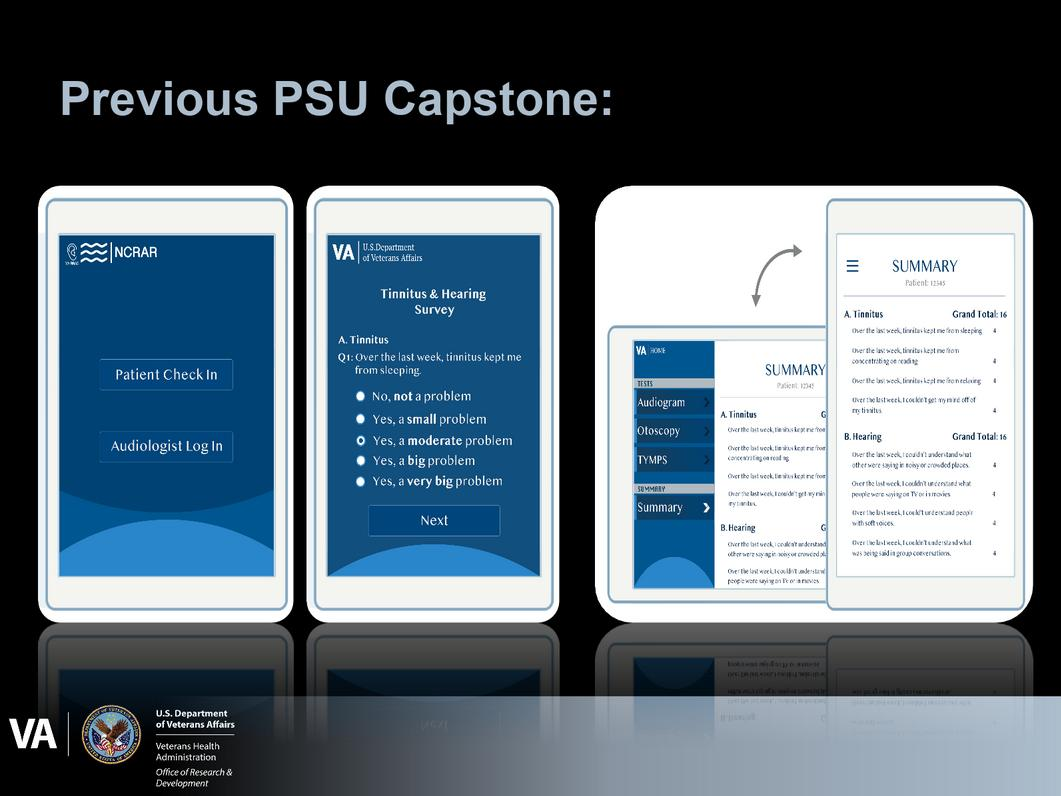
\includegraphics[width=0.8\linewidth]{P2-c.jpg}
\caption[VA]{VA}
\label{fig:VA}
\end{figure}	
\newpage
\begin{figure}[h!]
\centering
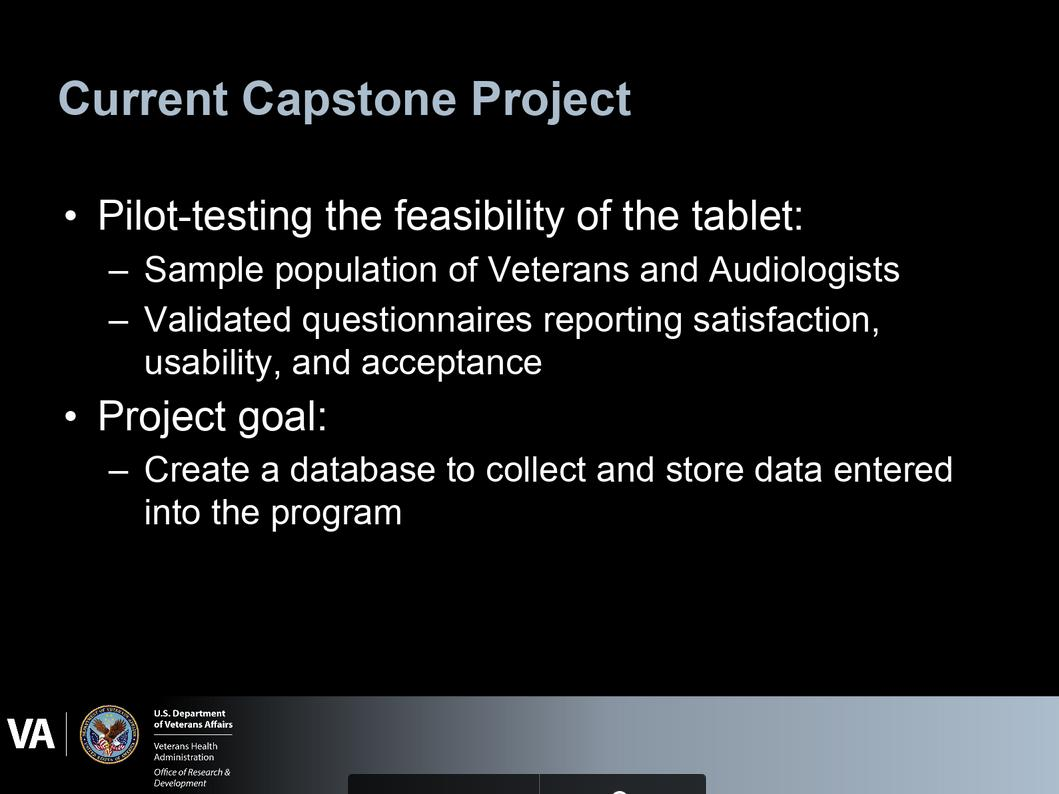
\includegraphics[width=0.8\linewidth]{P2-d.jpg}
\caption[VA]{VA}
\label{fig:VA}
\end{figure}	

\newpage
\section*{Development of a dashboard for selected Urban Key Performance Indicators}

Web based dashboard\\

It's proof of concept not actual product and data\\

\begin{figure}[h!]
\centering
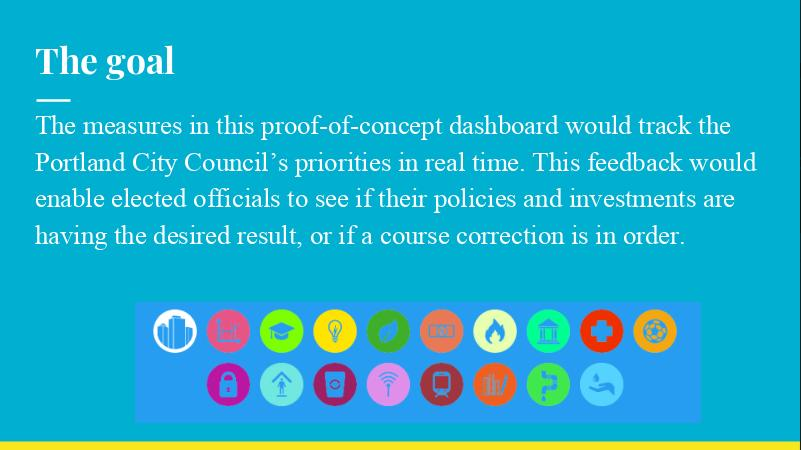
\includegraphics[width=0.8\linewidth]{P4-a.jpg}
\caption[City of Portland]{City of Portland}
\label{fig:City of Portland}
\end{figure}	

\begin{figure}[h!]
\centering
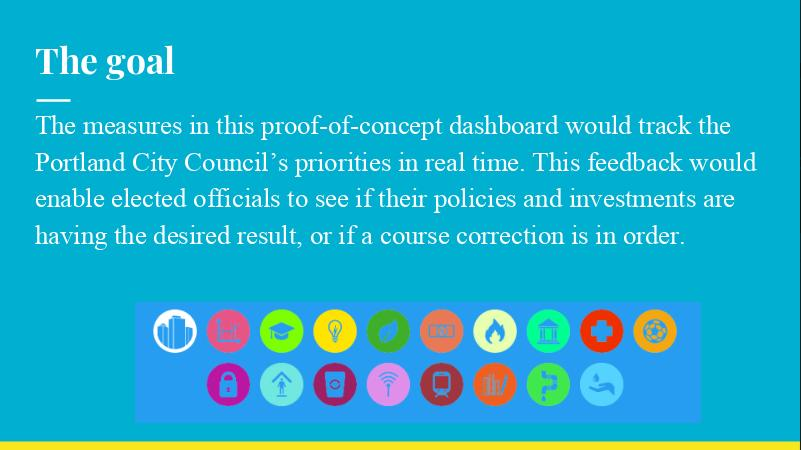
\includegraphics[width=0.8\linewidth]{P4-a.jpg}
\caption[City of Portland]{City of Portland}
\label{fig:City of Portland}
\end{figure}	

\newpage

\section*{Capstone 360 Review System}

\begin{figure}[h!]
\centering
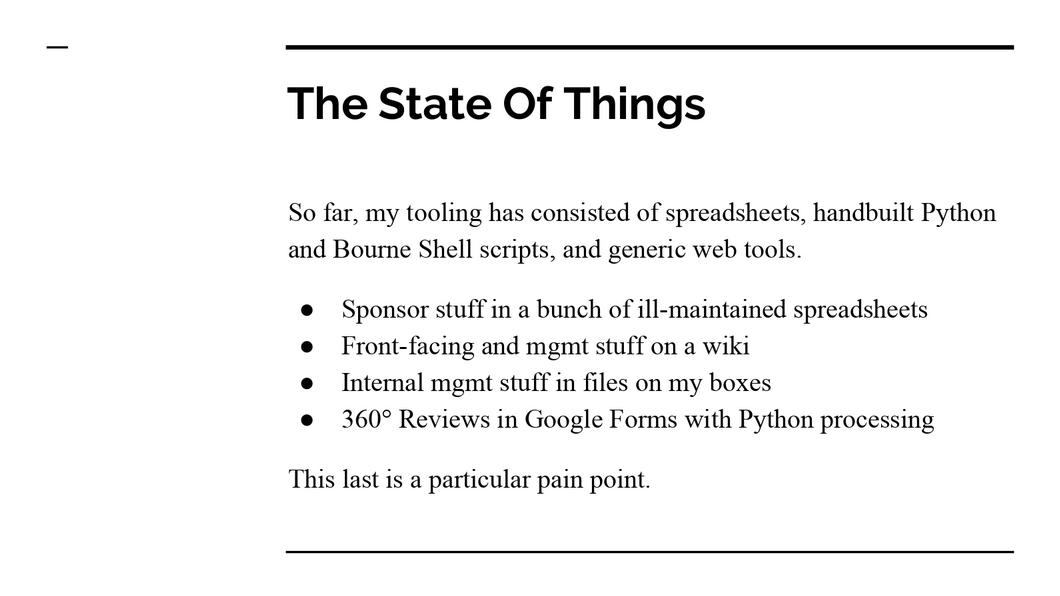
\includegraphics[width=0.8\linewidth]{P5-a.jpg}
\caption[PSU]{PSU}
\label{fig:PSU}
\end{figure}	

\begin{figure}[h!]
\centering
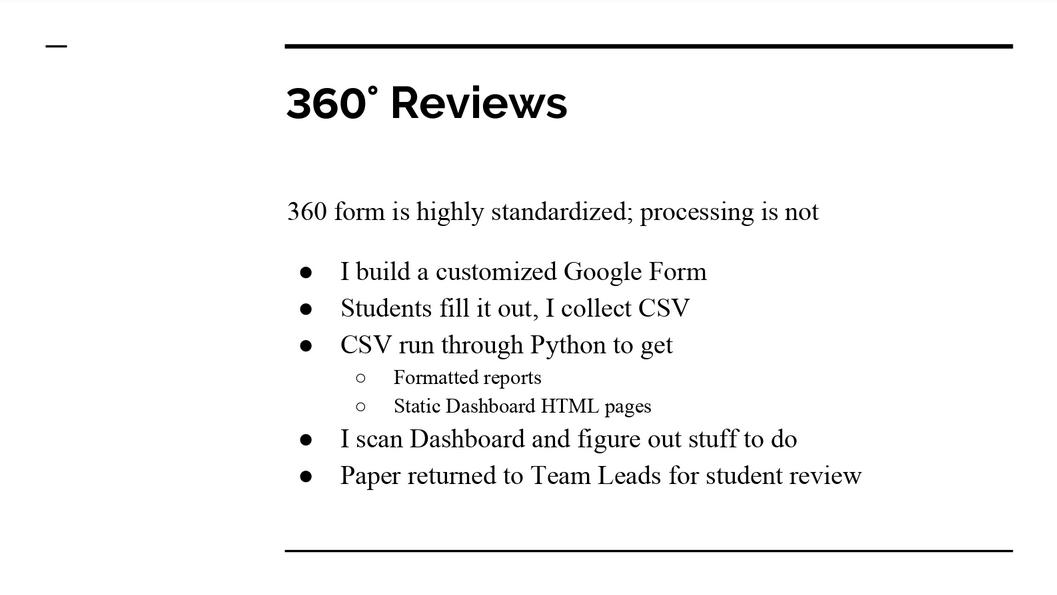
\includegraphics[width=0.8\linewidth]{P5-b.jpg}
\caption[PSU]{PSU}
\label{fig:PSU}
\end{figure}	
\newpage

\begin{figure}[h!]
\centering
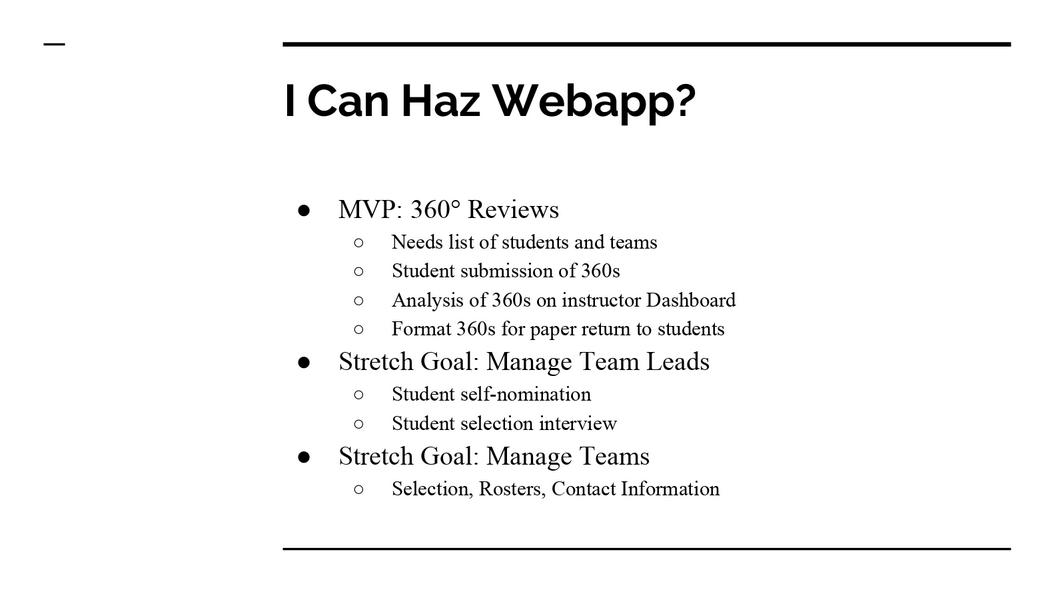
\includegraphics[width=0.8\linewidth]{P5-c.jpg}
\caption[PSU]{PSU}
\label{fig:PSU}
\end{figure}	


\begin{figure}[h!]
\centering
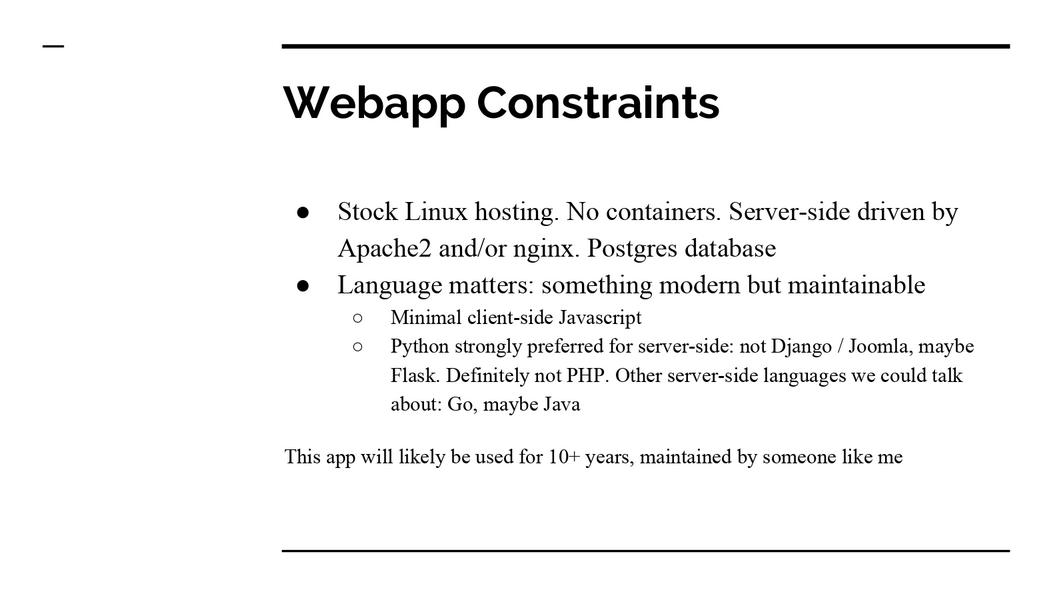
\includegraphics[width=0.8\linewidth]{P5-d.jpg}
\caption[PSU]{PSU}
\label{fig:PSU}
\end{figure}	
\newpage
\begin{figure}[h!]
\centering

\includegraphics[width=0.8\linewidth]{P5-e.jpg}
\caption[PSU]{PSU}
\label{fig:PSU}
\end{figure}	

\begin{figure}[h!]
\centering
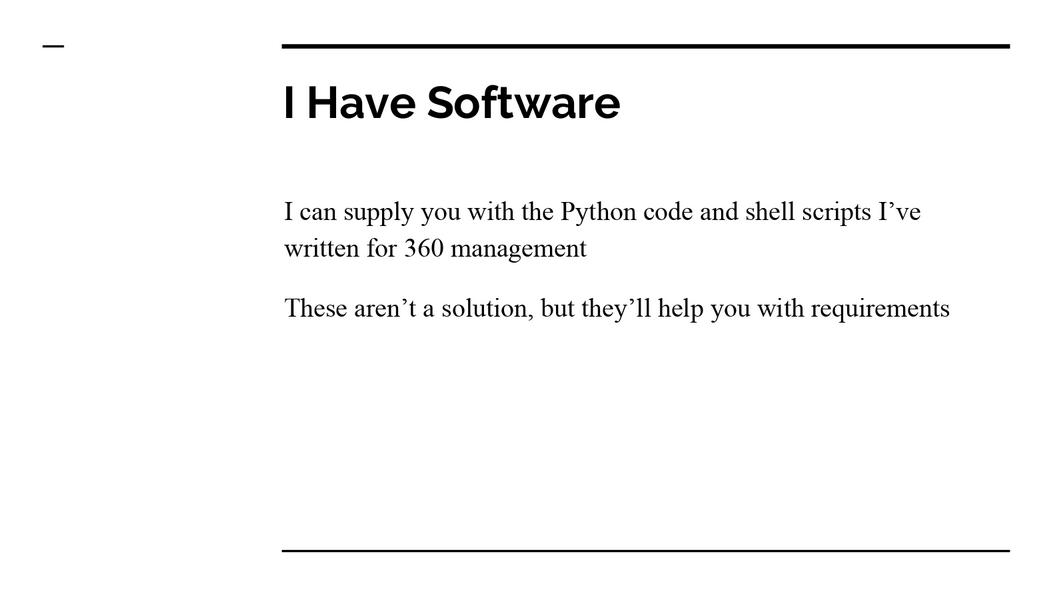
\includegraphics[width=0.8\linewidth]{P5-f.jpg}
\caption[PSU]{PSU}
\label{fig:PSU}
\end{figure}	
